%!TEX root = minta_dolgozat.tex
%%%%%%%%%%%%%%%%%%%%%%%%%%%%%%%%%%%%%%%%%%%%%%%%%%%%%%%%%%%%%%%%%%%%%%%
\chapter{User documentation}\label{ch:BASIC}
%%%%%%%%%%%%%%%%%%%%%%%%%%%%%%%%%%%%%%%%%%%%%%%%%%%%%%%%%%%%%%%%%%%%%%%

\begin{summary}
	In this chapter I describe the application from a user point of view.
\end{summary}

%%%%%%%%%%%%%%%%%%%%%%%%%%%%%%%%%%%%%%%%%%%%%%%%%%%%%%%%%%%%%%%%%%%%%%%
Here I describe the visuals of the application with images, 2-3 pages.

	\section{Greeting Page}

		The Greeting Page of the application consists of a frame containing a greeting message followed by two buttons: Login and Register.
		\begin{figure}[H]
			\centering
			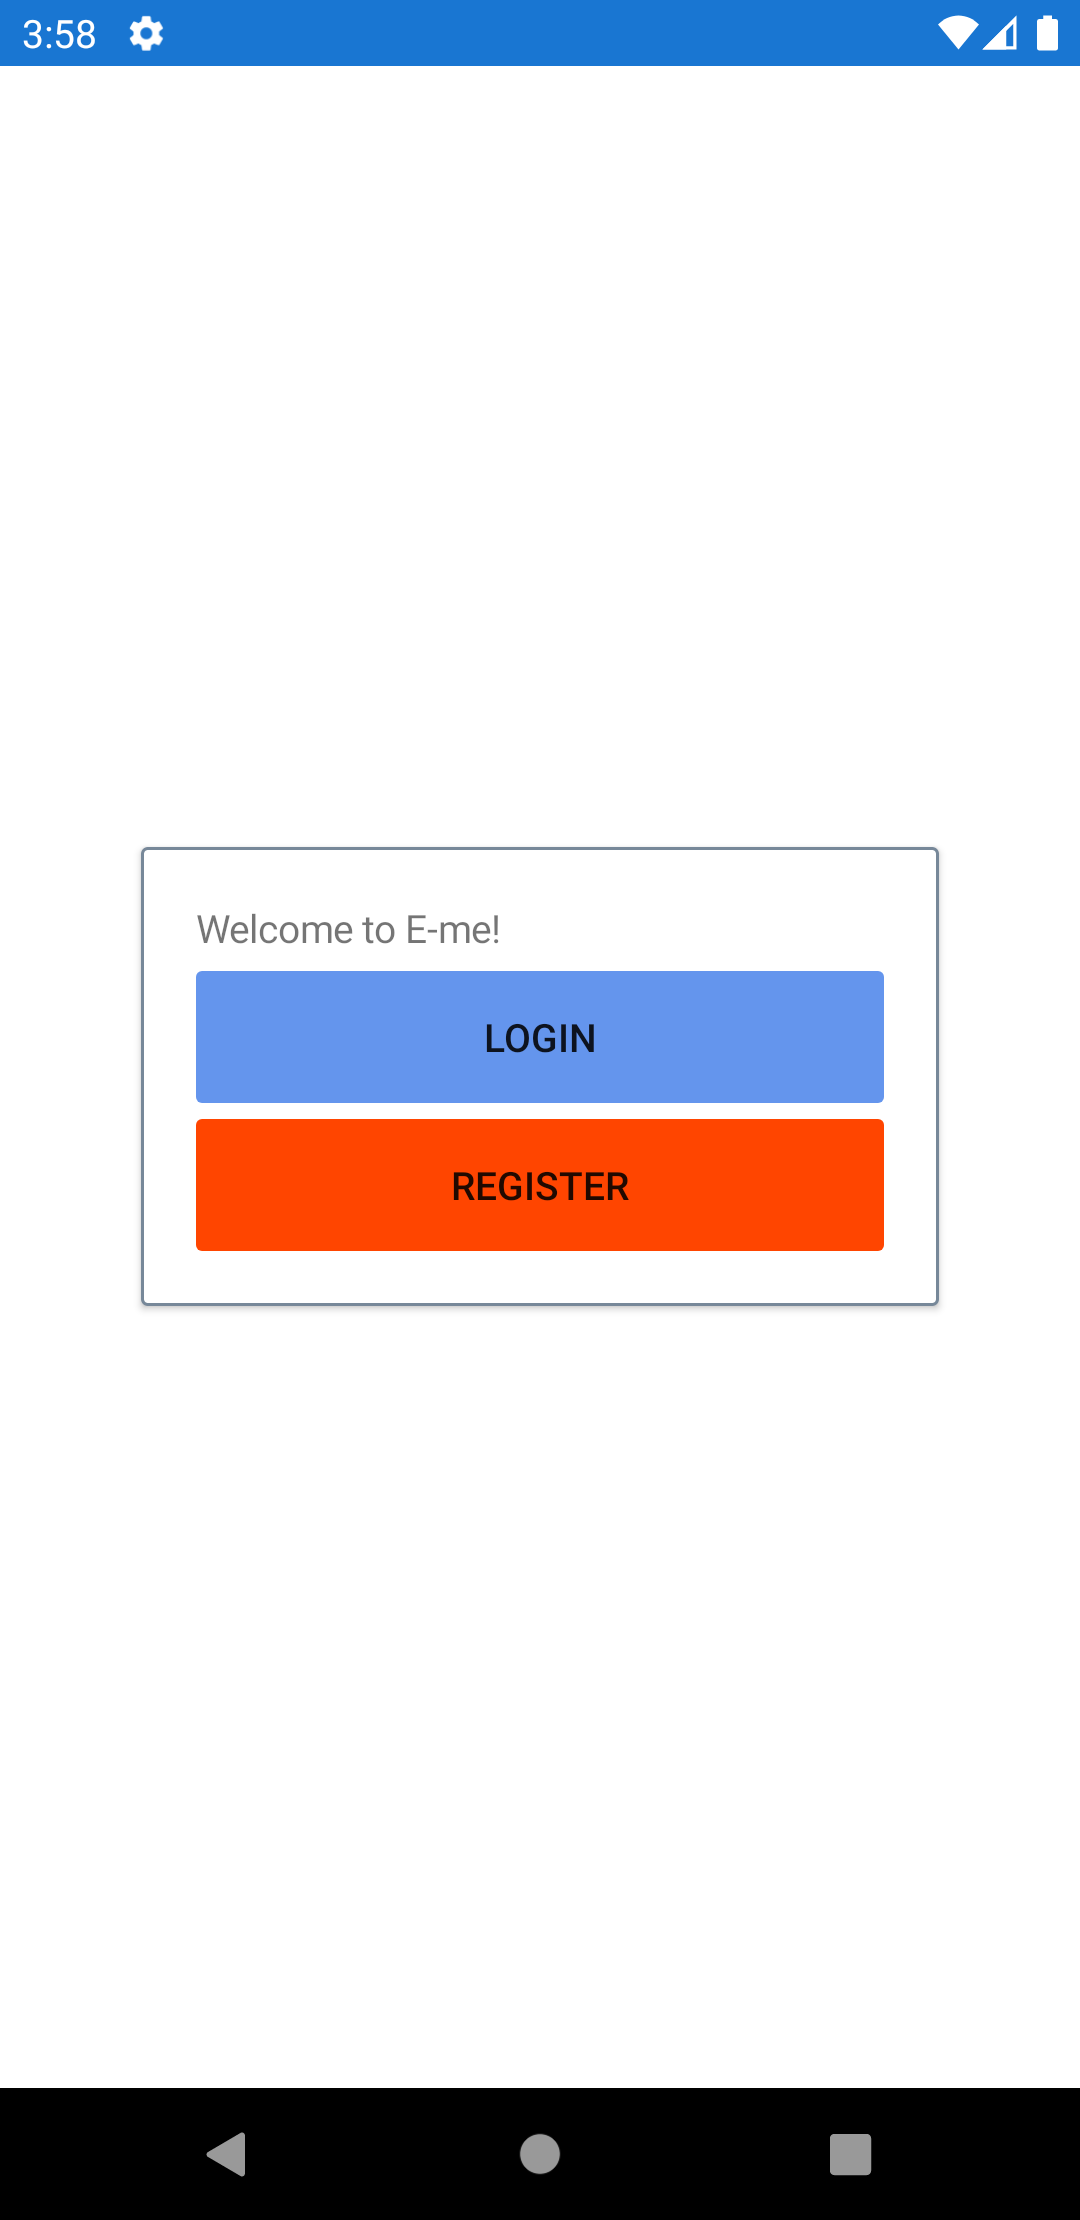
\includegraphics[scale=0.1]{main-page}				
			\caption{Greeting Page}
		\end{figure}
		These buttons allow the user to navigate to the Login Page and Registration Page respectively in order to authenticate themselves or create a new profile.

	\section{Registration Page}

	The Registration Page consists of a frame containing the registration form and a submit button (Register).
	The form contains five text fields which can be filled out by the user:
		\begin{enumerate}
			\item Full name
			\item Email
			\item Login name
			\item Password
			\item Confirm password
		\end{enumerate}

		\begin{figure}[H]
			\centering
			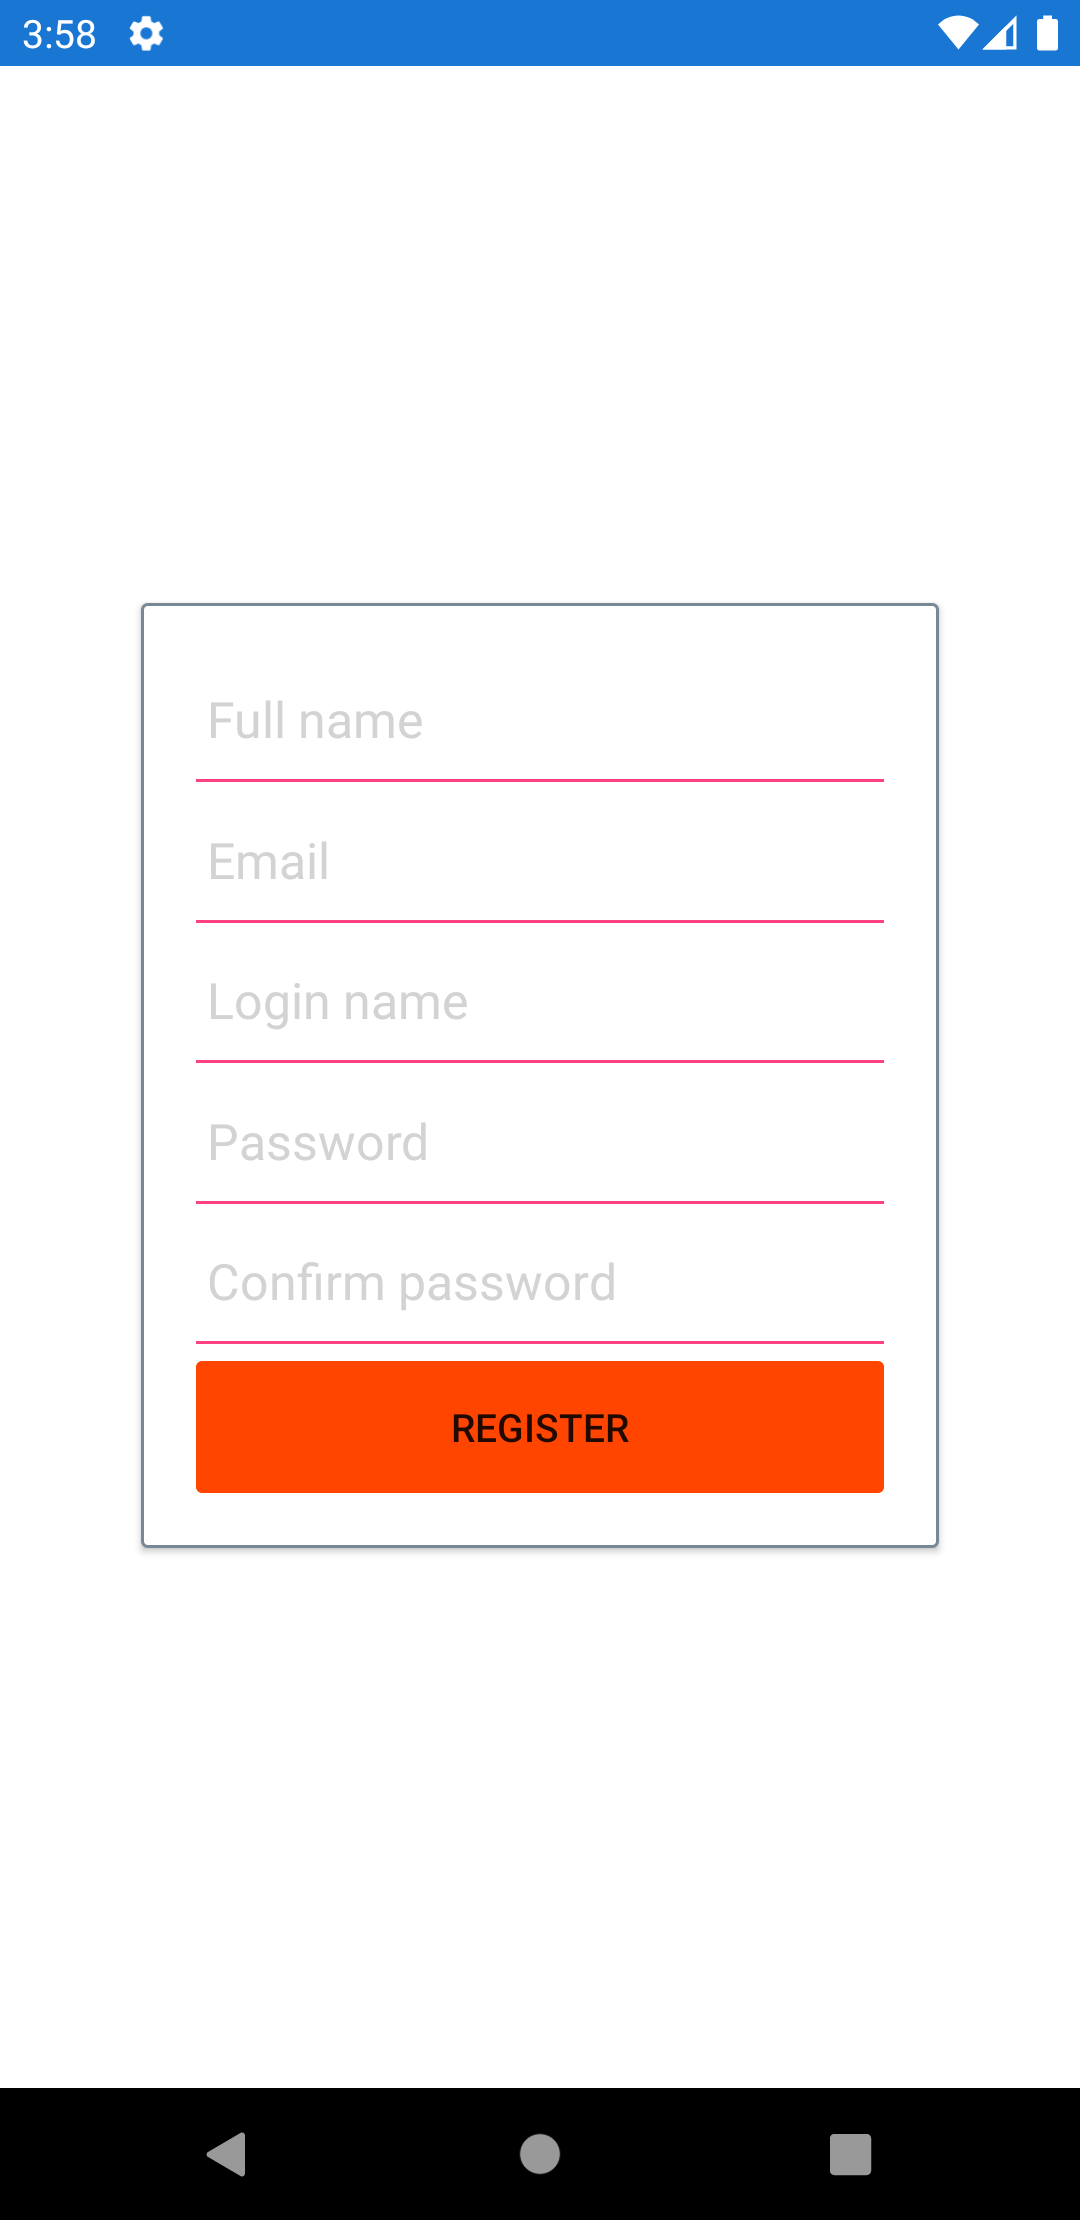
\includegraphics[scale=0.1]{register-page}				
			\caption{Registration Page}
		\end{figure}

	Every field is required in order to create a new user.
	Upon successful registration, the application navigates the user to the Login Page in order for them to authenticate themselves.

	\section{Login Page}

	The Login Page consists of a frame containing the login form and a submit button (Login).
	The form contains two text fields which can be filled out by the user:
		
		\begin{enumerate}
			\item Login name
			\item Password
		\end{enumerate}

		\begin{figure}[H]
			\centering
			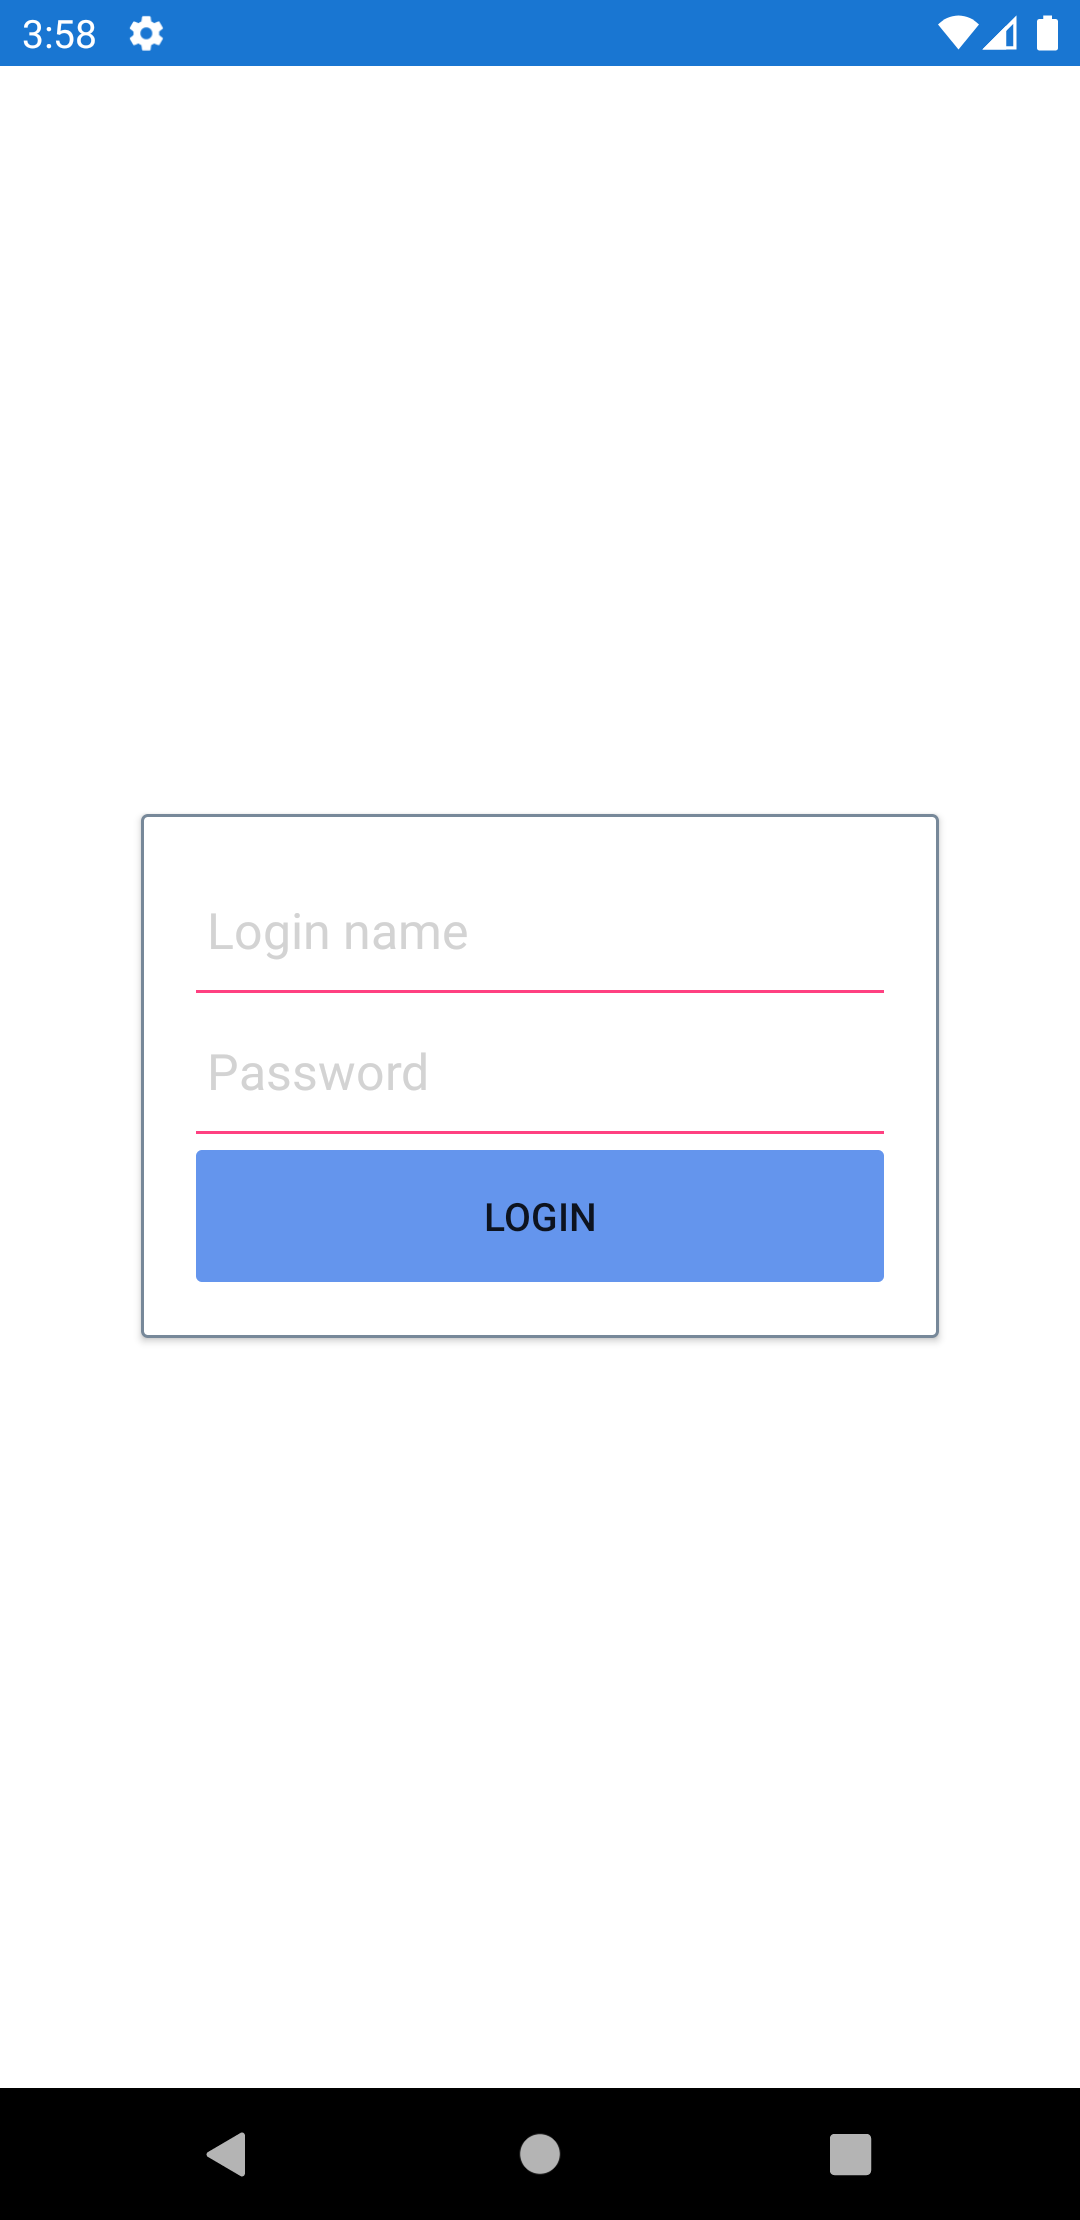
\includegraphics[scale=0.1]{login-page}				
			\caption{Login Page}
		\end{figure}

	Both fields are required in order to successfully authenticate a user.
	Upon successful login, the application navigates the user to the main tab menu where three tabs can be seen: My Documents, Request Document and Personal Info.

	\section{Documents Page}\label{documents}
	The Documents Page consists of two main parts: the list of documents and the "Scan QR code" button.

	The list of documents allows the user to visualize what types of documents they own.
	For each type the list contains the name of the document on the left and two buttons on the right: "Share" and "Remove".

	The "Scan QR code" button is a rounded floating element on the bottom right of the page which is always visible.

		\begin{figure}[H]
			\centering
			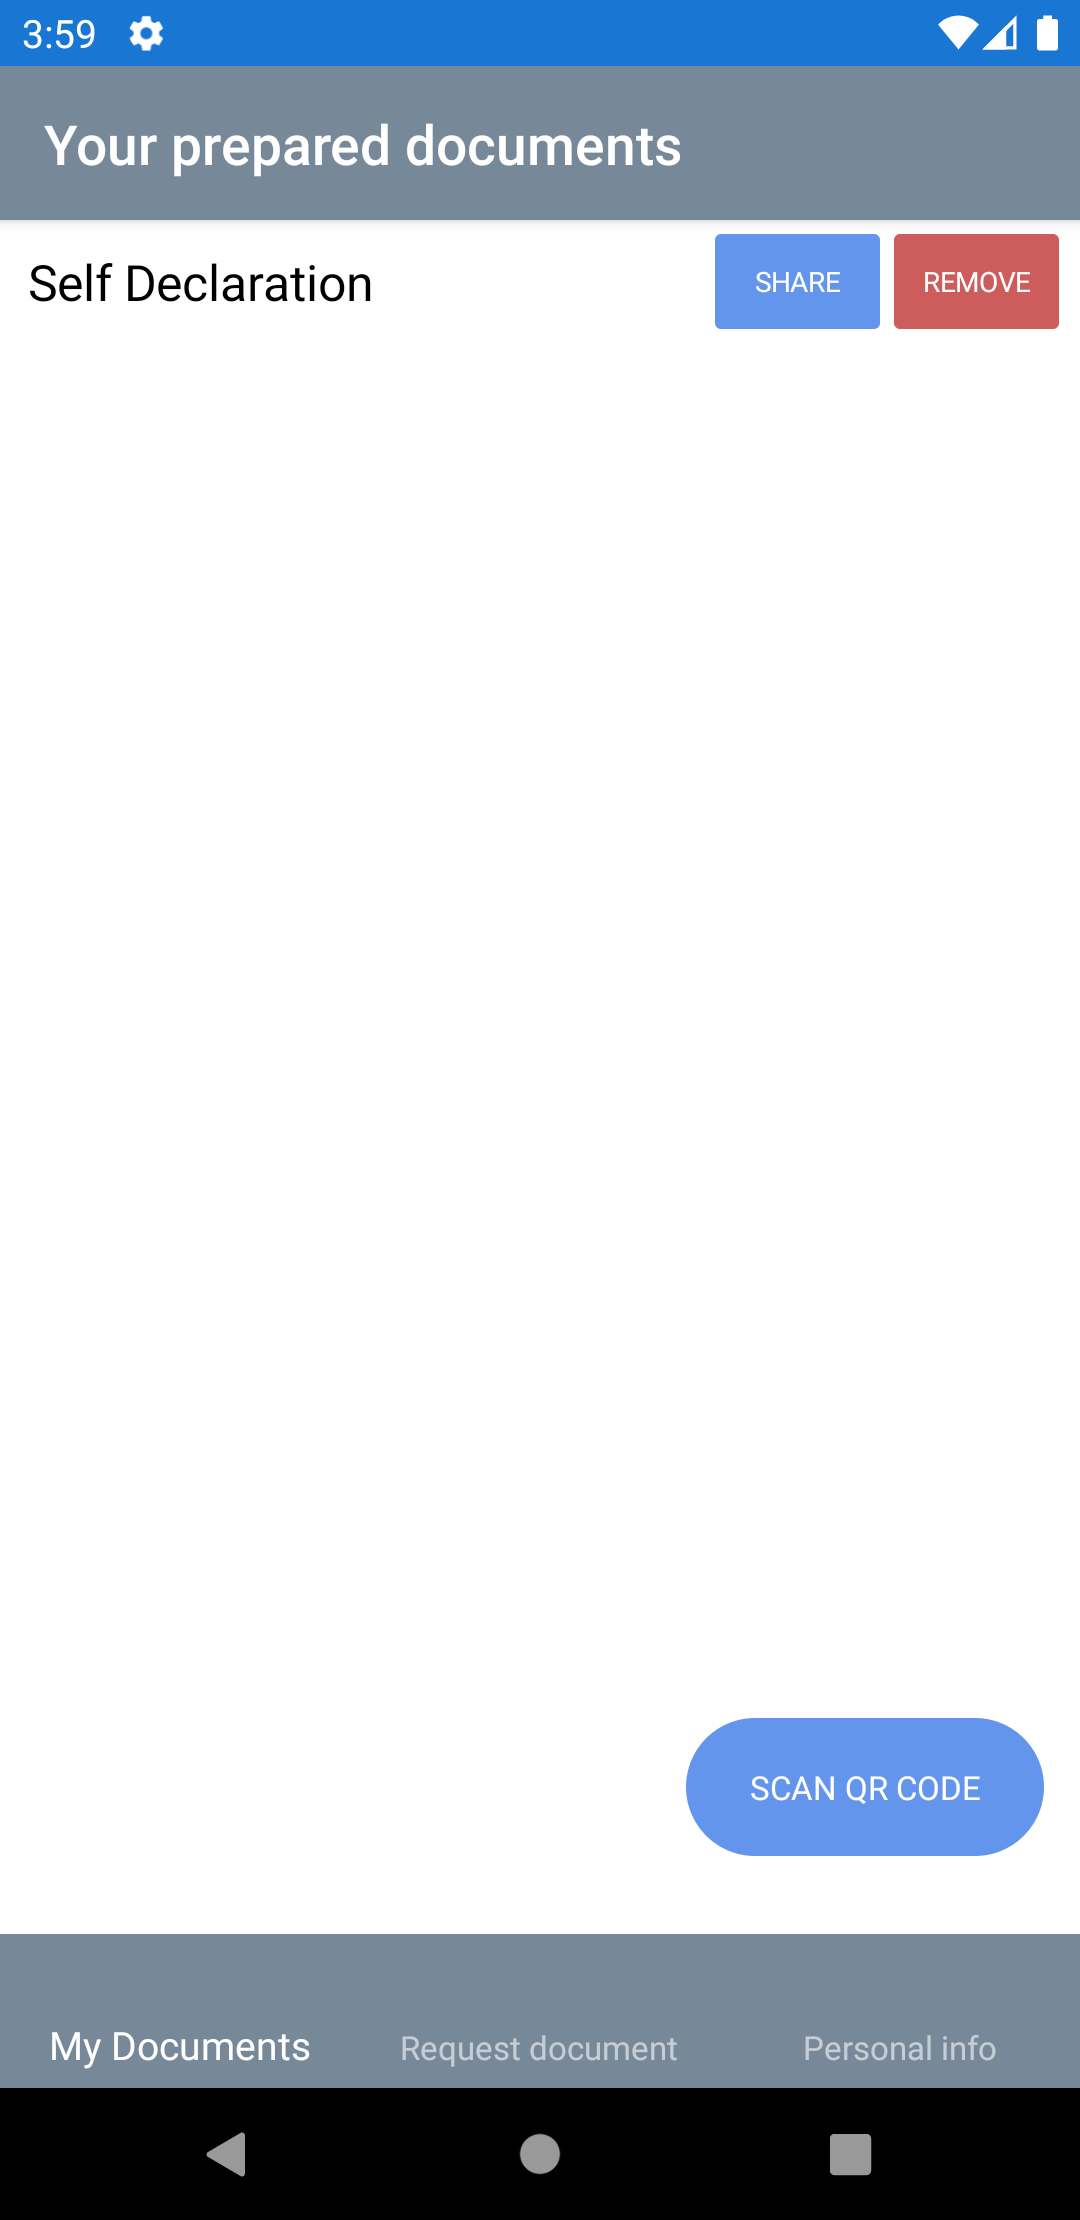
\includegraphics[scale=0.1]{documents-page}				
			\caption{Documents Page}
		\end{figure}

		Tapping the Remove button irreversibly deletes the document from the list.
		After a successful removal the user is able to request a new document of the same type, however if the document template was modified since
		the previous request or the user modified their personal information, the resulting document may be different than the previously deleted one.

		The Share button allows the user to safely transfer their selected document to a different device.
		Upon tapping the button, the application generates a unique code for the document which is then displayed on the screen via a QR code (see \hyperref[shareDocument]{Share Document Page}).

		The code mentioned above can be read using the "Scan QR code" button. 
		Tapping the button will attempt to open the device's main camera in order to scan the code.
		If this feature is accessed for the first time, a prompt appears asking for the user's permission to use the camera.
		If the permission is granted, the application will open the camera app. 
		Upon successfully reading a QR code generated by E-me, the selected document will appear on the screen (see \hyperref[document]{Document Page}).

	\section{Request Document Page}

	The Request Document Page consists of a list of document types that can be acquired by the user.
	The list only contains types that are not yet owned by user.
	If the user acquires one of these document types, it will not be shown on this page anymore (it will be listed on the \hyperref[documents]{Documents Page}).

	Together with the \hyperref[documents]{Documents Page}, these two pages contain every document type that can be managed through the application. 
		\begin{figure}[H]
			\centering
			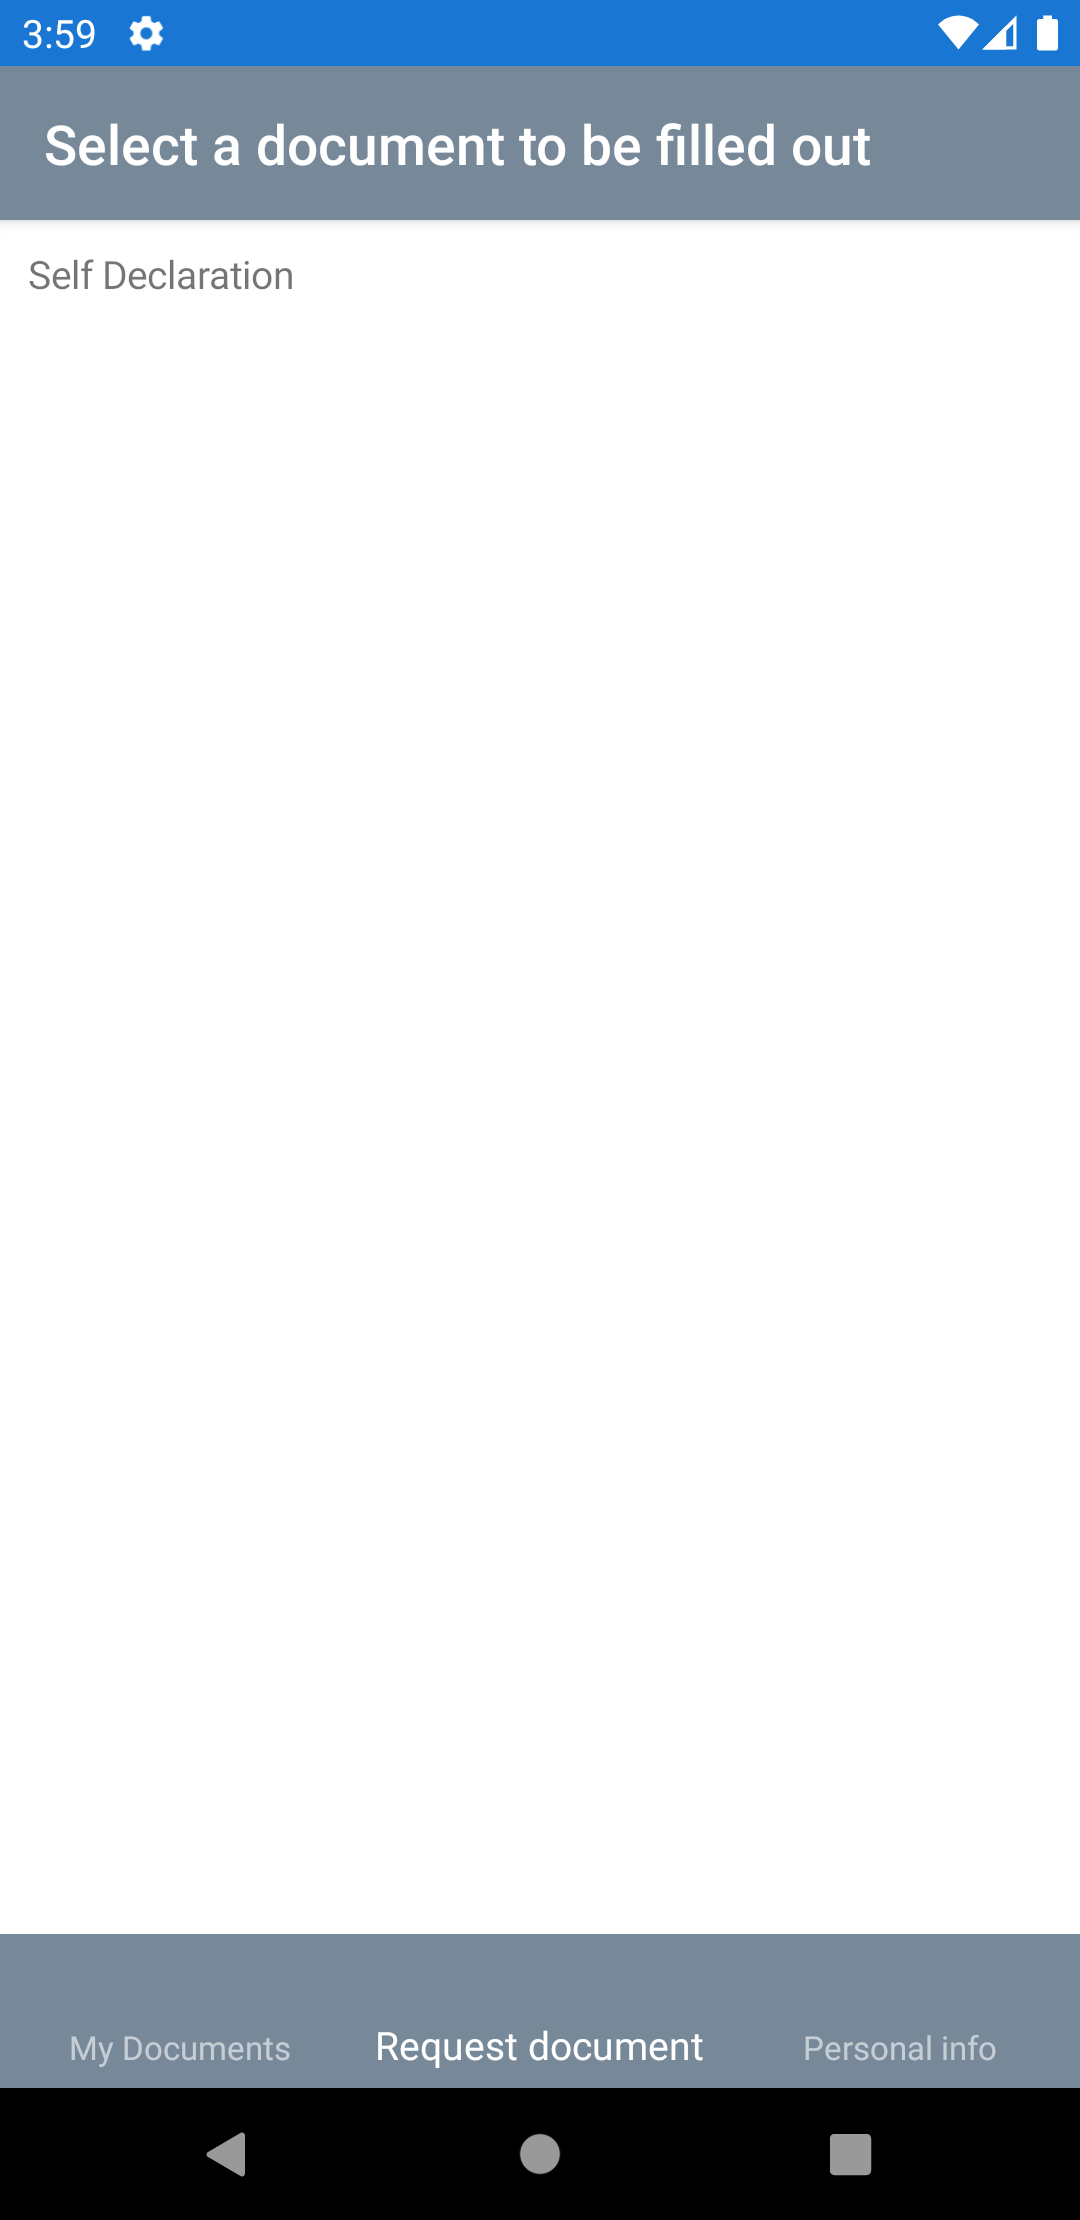
\includegraphics[scale=0.1]{request-document-page}				
			\caption{Request Document Page}
		\end{figure}

		The user can request a document by simply tapping on an item from the list (this action removes the selected item from this list). 
		The requested document will be generated and automatically displayed on the screen (see \hyperref[document]{Documents Page}).

	\section{Personal Information Page}

	The Personal Information Page consists of a form and a submit button (Save). 
	The form contains multiple text fields, date pickers, masked textboxes that can be filled out by the user.

	The submit button is located at the bottom of the page and is disabled until the user modifies at least one of the form fields.
		\begin{figure}[H]
			\centering
			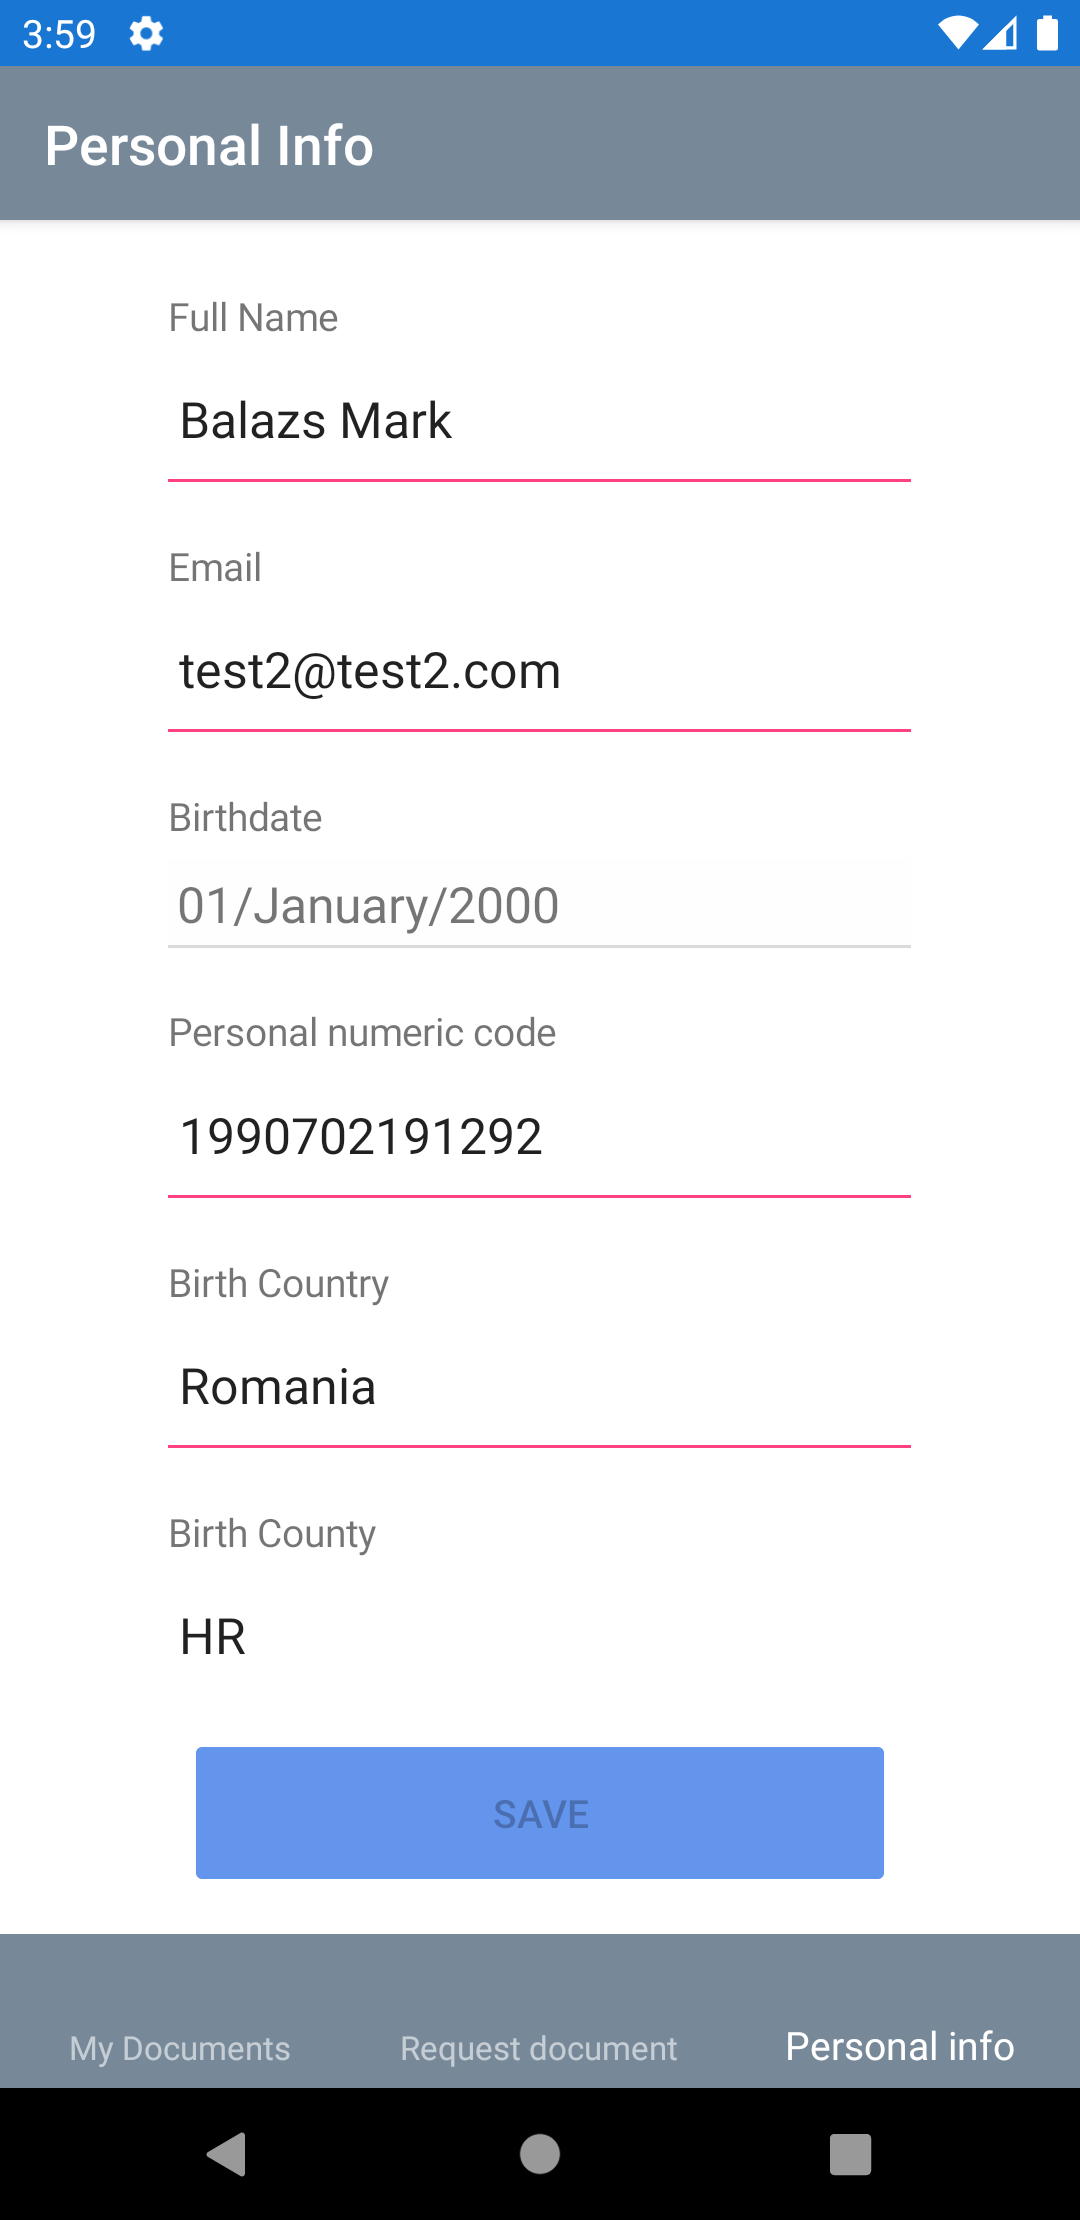
\includegraphics[scale=0.1]{personal-info-page}
			\caption{Personal Information Page}
		\end{figure}

		The information provided by the user on this page will be encrypted and stored by the application.
		Upon requesting a document, E-me attempts to match the fields of the document with the information of the user and fill them out respectively.
		Fields that require information that is not provided by the user will be left blank and can be filled manually on the \hyperref[document]{Document Page}.

	\section{Share Document Page}\label{shareDocument}

	The Share Document Page contains a short hint followed by a QR code in the middle of the screen.
	The code contains information about the document which was selected to be shared.
		\begin{figure}[H]
			\centering
			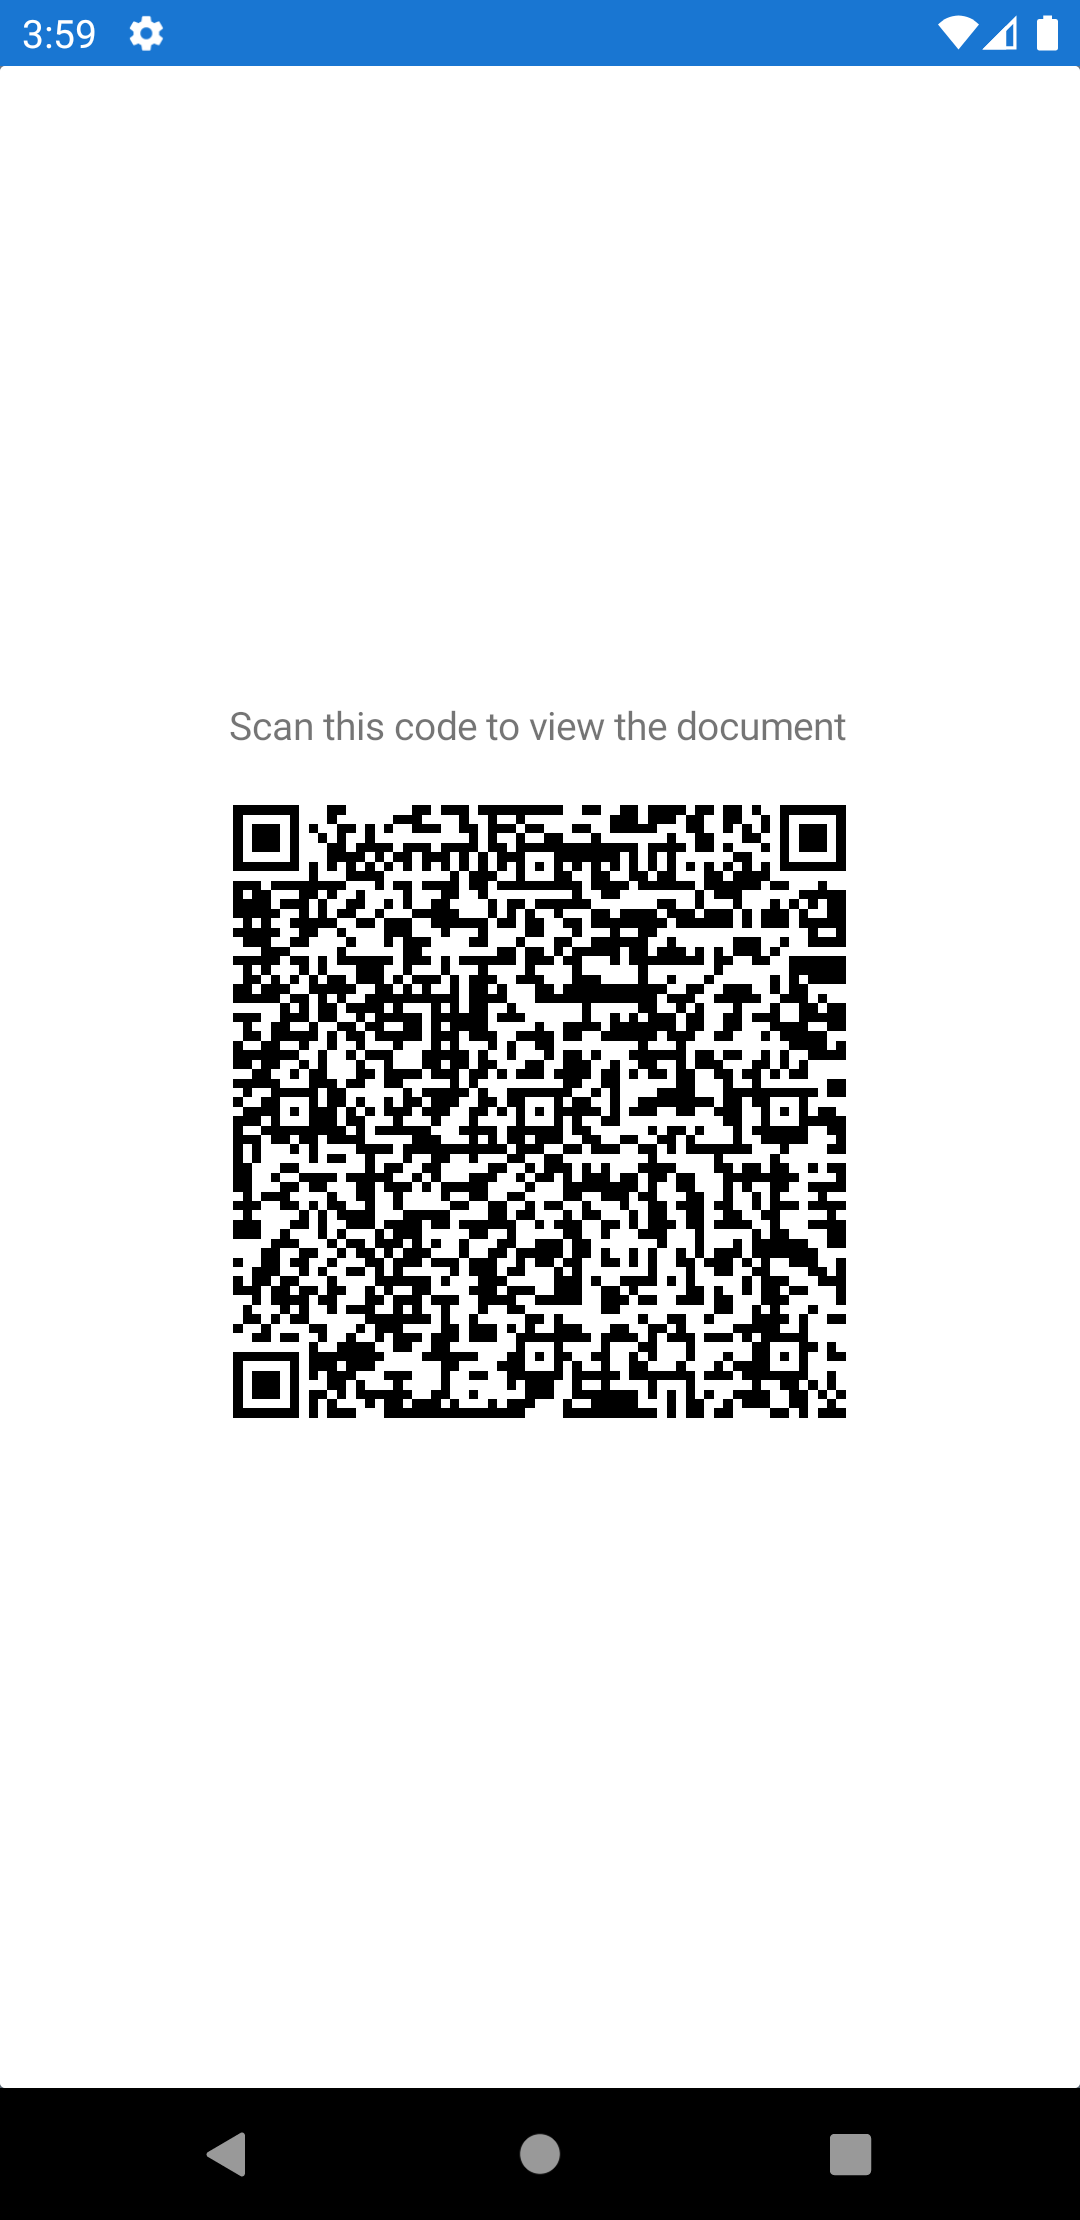
\includegraphics[scale=0.1]{share-document-page}
			\caption{Share Document Page}
		\end{figure}
	The user can return to the \hyperref[documents]{Documents Page} by pressing the Back button.

	\section{Document Page}\label{document}

	The Document Page is a PDF Viewer that consists of three parts: header menu, content and footer menu.
	The header menu contains four icons for saving, searching, printing and bookmark browsing in the opened PDF document.
	The content part of the viewer is the PDF itself which was generated and filled out by the application.
	The footer menu contains information about the number of pages that the document has, but also a drawer menu with actions for editing the opened document.
		\begin{figure}[H]
			\centering
			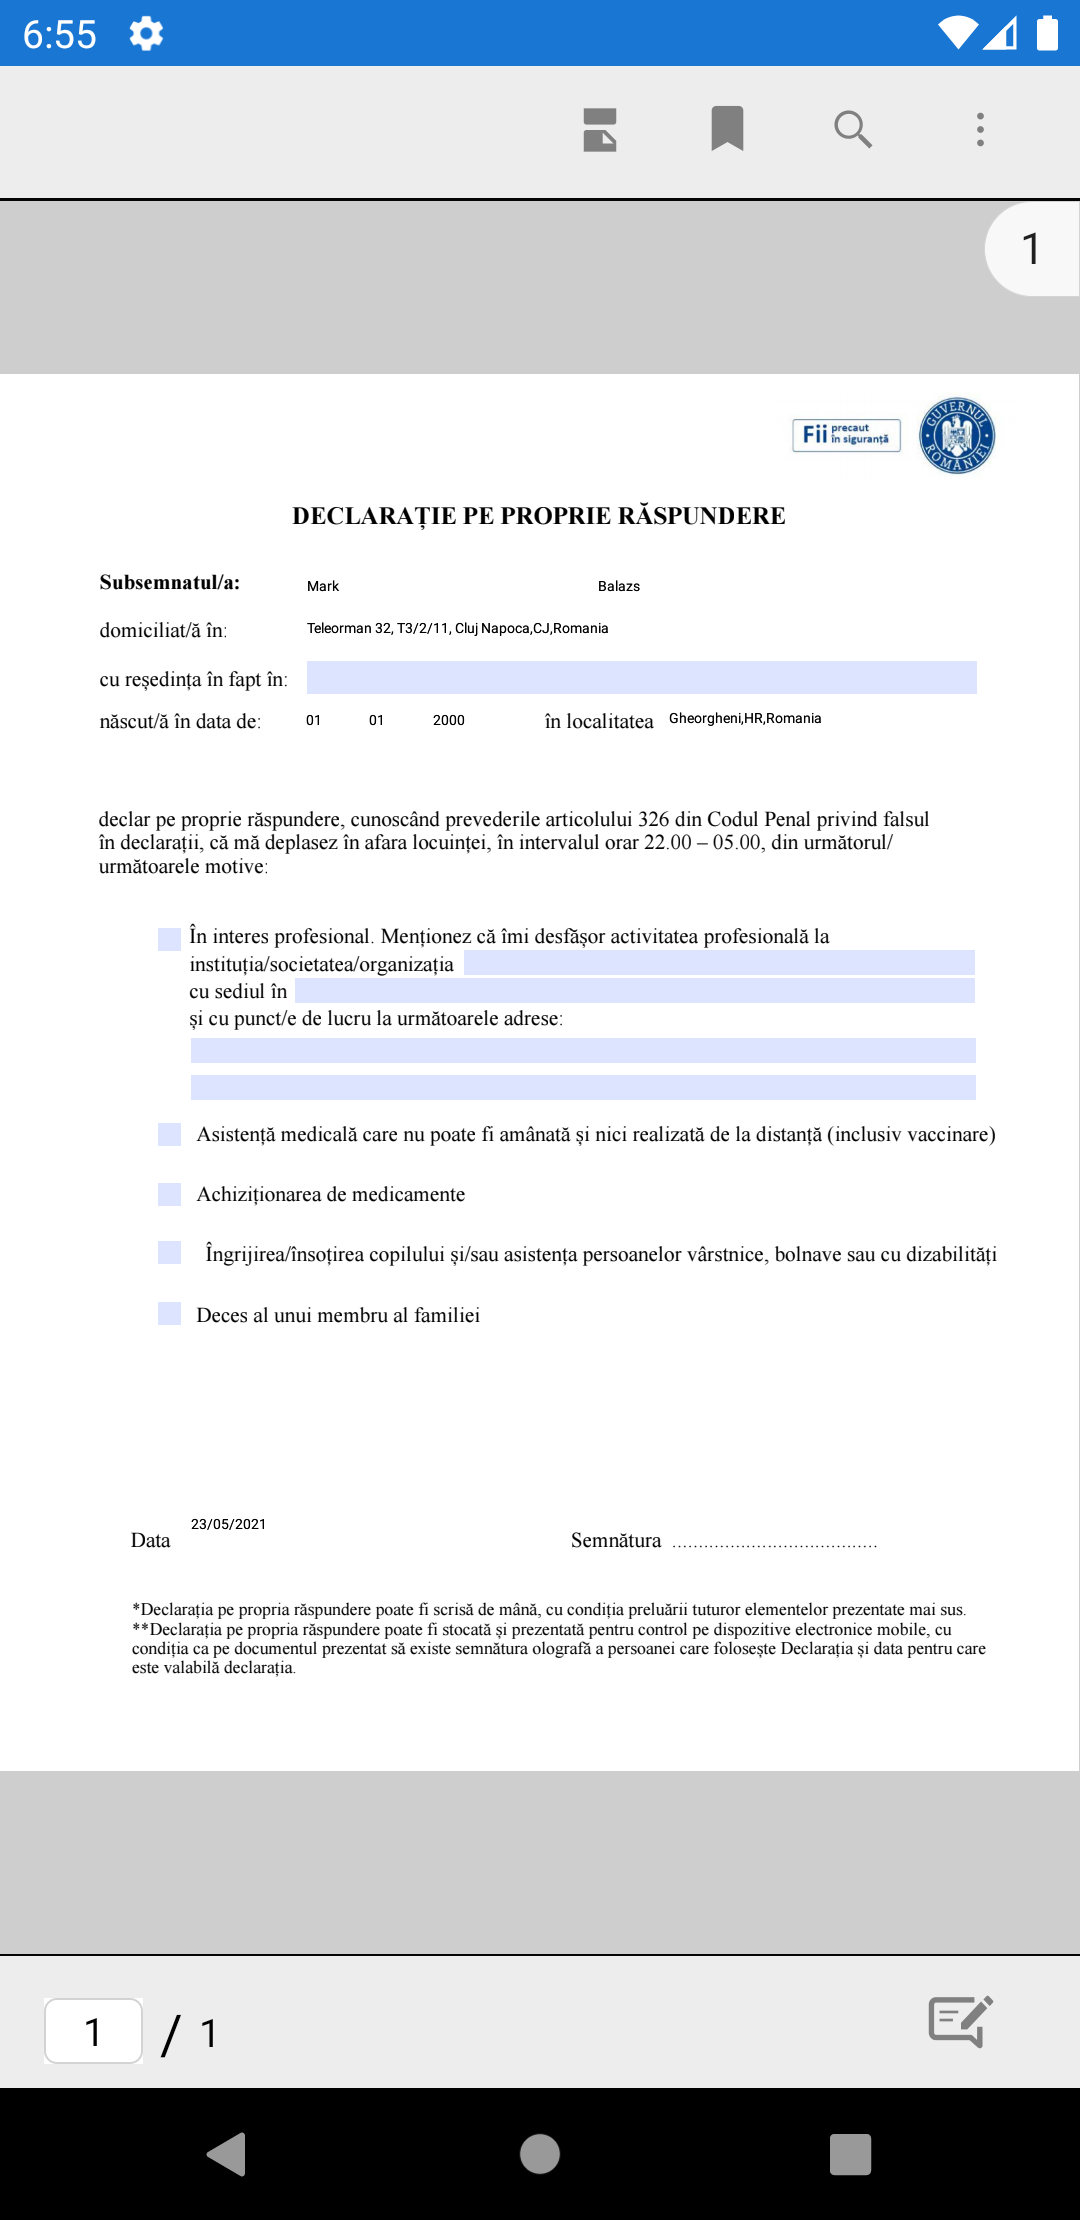
\includegraphics[scale=0.1]{document-page}
			\caption{Document Page}
		\end{figure}

	If the document contains form fields that were not filled automatically by the application, the user is able to fill them out manually.
	The document can be closed by pressing the Back button.